\documentclass[a4paper]{article} % This command is used to set the type of document you are working on such as an article, book, or presenation

\usepackage{geometry} % This package allows the editing of the page layout
\usepackage{subcaption}
\usepackage{amsmath}  % This package allows the use of a large range of mathematical formula, commands, and symbols
\usepackage{graphicx}  % This package allows the importing of images
\usepackage{fancyhdr}
\usepackage[hidelinks]{hyperref}
\usepackage[german]{babel}

\hypersetup{
    colorlinks=false, %set true if you want colored links
    linktoc=all,     %set to all if you want both sections and subsections linked
    linkcolor=blue,  %choose some color if you want links to stand out
}

\geometry{
  a4paper,
  left=20mm,
  right=20mm,
  headheight=5cm,
  top=3.5cm,
  bottom=2.5cm,
  footskip=0.5cm
}

\pagestyle{fancy}                    % Eigener Seitenstil
\fancyhf{}                           % Alle Kopf- und Fußzeilenfelder bereinigen
\fancyhead[L]{SL1}          % Kopfzeile links
\fancyhead[C]{SE1 SS23}                      % Zentrierte Kopfzeile
\fancyhead[R]{Pilotenlogbuch}                  % Kopfzeile rechts
\renewcommand{\headrulewidth}{0.4pt} % Obere Trennlinie
\fancyfoot[R]{\thepage}              % Seitennummer
\renewcommand{\footrulewidth}{0.4pt} % Untere Trennlinie

\newcommand{\source}[1]{\caption*{Quelle: {#1}} }

\newcommand*{\captionsource}[2]{%

    \caption[{#1}]{%
        #1%
        \\\hspace{\linewidth}%
        \centering\textbf{Quelle:} #2%
    }%
}

\newcommand{\question}[2][]{\begin{flushleft}
        \textbf{Frage #1}: \textit{#2}

\end{flushleft}}
\newcommand{\sol}{\textbf{Solution}:} %Use if you want a boldface solution line
\newcommand{\maketitletwo}[2][]{\begin{center}
        \vspace*{50pt}

        \Huge{\textbf{Studienleistung 1}

            SE1-SS23} % Name of course here
        \vspace{5pt}
        
        \Large{\today}
        \vspace{350pt}

        \vspace{15pt}
        
    \end{center}

    \begin{flushleft}
        \normalsize\Large{
            \textbf{Gruppenarbeit von:}\\Mohammad Hawrami (2210970)\\Cedric Hermann (2210943)\\Philipp Kotte (2211945) % Your name here
        }  
    \end{flushleft}
}



\begin{document}

    \maketitletwo[1]  % Optional argument is assignment number
    %Keep a blank space between maketitletwo and \question[1]
    
    \pagebreak

    \vspace*{10pt}
    \tableofcontents

    \pagebreak

    \section{Problem des Kunden}
    \vspace{1cm}
    Kundenseite:\\
    Als Entwickler eines Programmes oder einer App ist es von größter Wichtigkeit, dass man die Bedürfnisse seines Auftraggebers genau kennt, um ihm das bestmögliche Produkt zur Verfügung stellen zu können. In diesem Fall möchte unser Kunde sein etwas veraltetes und altmodische Flug-Logbuch loswerden und durch eine modernere und digitale App ersetzen.\\
    Einer der Hauptgründe, warum unser Kunde das altmodische Flug-Logbuch nicht mehr benutzen möchte, ist die Tatsache, dass er es nicht digital verfügbar hat. Dies hat in der Vergangenheit immer wieder zu Problemen geführt, wenn er sein Logbuch vergessen hatte oder er dieses gar nicht mehr an dem Flug tag fand.\\
    Mit der neuen App möchte er außerdem eine hohe Verfügbarkeit über das Digitale Flug-Logbuch besitzen, damit er jederzeit und überall auf dieser Welt darauf zurückgreifen kann, um seinen neunen Daten einzutragen oder die etwas älteren aufzurufen.\\
    Ein weiteres Problem mit dem veralteten System ist die unübersichtliche Gestaltung des Flug-Logbuches. Unser Kunde möchte immer einen klaren Überblick über seine aktuellen und vergangen Flüge haben. Er möchte zu dem auch in der Lage sein, alle benötigten Informationen auf einen Blick sehen zu können, ohne dass er ständig blättern muss. Daher ist es von größter Wichtigkeit, dass die neue App übersichtlich gestaltet ist und alle wichtigen Informationen klar und deutlich zu erkennen sind.\\
    
    \noindent Ein weiterer wichtiger Punkt für den Kunden ist die Speicherung aller Daten. Unser Kunde möchte alle wichtigen Informationen zu seinen Flügen gespeichert haben, wie beispielsweise Flugrouten, Datum und Dauer der Flüge sowie die Gültigkeit der Lizenzen. Diese Daten sollten wiederrum jederzeit abrufbar sein, damit unser Kunde schnell und einfach die benötigten Informationen finden kann.
    Schließlich ist es für unseren Kunden auch sehr wichtig, dass er bei Bedarf das Flug-Logbuch im Papierformat ausdrucken kann. Dies ist insbesondere dann hilfereich, wenn der Kunde beispielsweise seine Daten mit anderen Piloten teilen möchte oder wenn er eine Physische Kopie von dem Flug-Logbuch benötigt.\\
    Zusammenfassend möchte unser Kunde eine alternative zu dem veralteten System, wo er auch wiederum paar Anforderung hat, die er bei dem alerten System vermisst, beziehungsweise diese nicht vorhanden sind, oder diese sehr schlecht umgesetzt sind.\\  
    \vspace{0.5cm}\\
    \noindent Entwickler:\\
    Als Entwickler der App haben wir unserem Kunden noch paar Fragen gestellt, um sicherzustellen, dass wir seinen Bedürfnissen auch nachkommen können und gleichzeitig seine gewünschte App so entwickeln können, wie er sie haben möchte. Eine der Fragen war ob die App nur auf iOS laufen soll oder ob es auch wichtig ist, dass sie auch für Android-Nutzer funktionieren soll und bereitgestellt wird.\\
    
    \noindent Kunden Antwort:\\
    Der Kunde hat uns dazu eine klare Antwort gegeben. 
    Er möchte, dass so viele Piloten wie möglich die vereinfachte und digitale Version des Flug-Logbuches nutzen können. Aus diesem Grund was sein Verlangen, dass die App für jedes Betriebssystem erstellen werden sollte, egal ob die Piloten ein Android-Smartphone oder ein iOS-Gerät nutzen.\\
    \pagebreak
    \vspace{1cm}\\
    \noindent Entwickler:\\
    Eine weitere wichtige Frage war, ob sie nur für Mobilgeräte optimiert werden sollte oder ob es auch sinnvoll wäre, die App auch für andere Geräte zu erstellen, wie zum Beispiel für den Computer, Smartphone oder auch für iPad/Tablets.\\
    
    \noindent Kunden Antwort:\\
    Der Kunde möchte von uns eine hohe Verfügbarkeit. 
    Das heißt, die App sollte zumindest auf den gängigen Geräten laufen, wie auf dem Computer, Handy oder auch auf dem iPad/Tablet.Für den Kunden sollte es egal sein an, von welchem Gerät aus man gerade seine Daten einträgt.\\
    \vspace{0.5cm}\\
    \noindent Entwickler:\\
    Ein weiterer sehr wichtiger Punkt ist der Schutz vor fremden Personen, die Zugriff auf den Rechner unseres Kunden haben. Aus diesem Gründen haben wir unseren Kunden gefragt welche Sicherheit Möglichkeiten, es geben sollte damit mit an genau fremde Zugriffe untersagen kann. Heißt, sollte die App nur Passwort geschützt sein, oder solle es auch Biometrische-Funktionen besitzen, wie den Fingerabdruck oder die Gesicht Erkennung.\\
    
    \noindent Kunden Antwort:\\
    Auf unsere Frage zur Sicherheit hinsichtlich der Verschlüsselung der Daten und des Flug-Logbuches hat uns der Kunde erklärt, dass die Sicherheit für ihn eine hohe Priorität hat, da er nicht möchte, dass jemand einfach an seinen Rechner geht und seine Daten verändert. Außerdem meinte er, dass nicht nur die neusten Geräte von den Sicherheitsmaßnahmen profitieren sollte, sondern auch Nutzer, die beispielsweise ein älteres Smartphone bedienen, das keine Biometrie-Funktionen hat, sondern nur eine Passwort-Darstellung.\\
    \vspace{0.5cm}\\
    \noindent Entwickler:\\
    Eine der wichtigsten Fragen, die wir unserem Kunden gestellt haben, war, wie das Design der App aussehen soll, um sicherzustellen, dass es eine klare Übersichtlichkeit gibt und alle Funktionen leicht zugänglich für den Kunden sind.\\
    
    \noindent Kunden Antwort:\\
    Die Antwort unseres Kunden auf unsere Frage war simpel: Das Design des Flug-Logbuches sollte ähnlich aussehen wie das der altmodischen Variante, damit es zu keinen Missverständnissen kommen kann. Das Flug-Logbuch sollte in einem Tabellenformat gehalten sein. Die Bedingung der ganzen App sollte so gestaltet sein, dass sowohl die jüngeren als auch die ältere Generation die App problemlos bedienen kann. Es sollten keine komplizierten Wege zu der Kategorie geben, die man gerade aufrufen möchte, sowie einen sehr einfachen Weg, um Daten zu speichern.\\
    \pagebreak
    
    \section{Pflichtenheft}
    \vspace{1cm}
    \subsection{Zielbestimmung}
    Das Fluglogbuch ist eine Applikation, die einem Piloten ermöglicht, all die Daten die er Vor und Nach einem Flug aufschreiben muss, in der App zu speichern. Außerdem kann er dort weitere Daten hinterlegen, die ihm von Nutzen sein könnten wie zum Beispiel seine Fluglizenz.\\
    Im Folgenden bezeichnet \grqq{}Benutzer\glqq{} sowohl Männer als auch Frauen.\\
    
    \subsubsection{Muss Kriterien}
    \vspace{0.5cm}
    \begin{itemize}
    \item Mehrere Seiten für eine gute Übersicht
    \item Der Benutzer kann über alle Seiten beliebig navigieren
    \item Auflistung von Daten in Tabellenform
    \item Der Benutzer kann einen Eintrag in der Tabelle generieren
    \item Der Benutzer soll in der Lage sein den Eintrag den er gerade generieren will abzubrechen
    \item Der Benutzer soll die Tabelle drucken können
    \item Alle eingegeben Informationen sollen gespeichert werden können
    \end{itemize}

    \subsubsection{Wunschkriterien}
    \vspace{0.5cm}
    \begin{itemize}
    \item Der Benutzer kann eine Papierische Tabelle in die App übertragen lassen
    \item Bearbeitung von geschriebenen Spalten in einer Tabelle
    \end{itemize}
    
    \subsubsection{Abgrenzungskriterien}
    \vspace{0.5cm}

    \begin{itemize}
        \item Keine Validierung, ob eingegebene Werte im korrekten Format sind
        \item Alle Daten werden nur auf dem jeweiligem Endgerät gespeichert
        \item Keine Speziellen Datum Auswahlfelder, die müssen vom Benutzer auch eingegeben werden
    \end{itemize}
    \pagebreak
    
    \subsection{Produktfunktionen}
    \vspace{1cm}
    \begin{itemize}
        \item \textbackslash F0010\textbackslash{} Speicherung: \\
        \noindent \\Alle Informationen aus Tabellen sollen auf dem Endgerät gespeichert werden, sodass die Tabellen erhalten bleiben, auch wenn der Benutzer die App zwischendurch schließt.\\\vspace{0.5cm}
        \item \textbackslash F0020\textbackslash{} Neuen Eintrag:\\
        \noindent \\Neue Zeilen in einer Tabelle anlegen ist das wichtigste in der App und soll einfach durch einen Knopf druck funktionieren.\\\vspace{0.5cm}
        \item \textbackslash F0030\textbackslash{} Eintrag erstellen: \\
        \noindent \\Eine neue Seite auf der man alle Informationen für den Neuen Tabellen Eintrag eingeben muss und dann auf der Seite Bestätigen drücken kann.\\\vspace{0.5cm}
        \item \textbackslash F0040\textbackslash{} Abbrechen: \\
        \noindent \\Der Button soll den Benutzer wieder auf die Logbuchseite führen.\\\vspace{0.5cm}
        \item \textbackslash F0050\textbackslash{} Drucken:\\
        \noindent \\Der Benutzer soll jeder Zeit die Option haben, die Tabellen zu drucken.\\\vspace{0.5cm}
    \end{itemize}
    \pagebreak
    \subsection{Produktdaten}
    \vspace{1cm}
    Im folgenden sind alle Daten die in der App gespeichert werden sollen mit dem zugehörigen Format aufgelistet.
    \vspace{0.5cm}
    \begin{itemize}
        \item Log\\
        \textbackslash D0010\textbackslash{} Sind alle Daten die für einen Logeintrag gebraucht werden.
        \begin{itemize}
            \item Datum
            \item Kennzeichen
            \item Flugzeugtyp
            \item Abflugsort
            \item Ankunftsort
            \item Ankunftsszeit
            \item Flugzeit SEP
            \item Flugzeit UL
            \item Landungen
            \item Operational Condition Night
            \item Flugzeit PIC
            \item Flugzeit Dual
        \end{itemize}
        \item Logbuch\\
        \textbackslash D0020\textbackslash{} sind alle Daten die man generell für das Logbuch benötigt.
        \begin{itemize}
            \item Vorname
            \item Nachname
            \item Anschrift
            \item Geburtsdatum
            \item Geburtsort
            \item Nationalität
            \item Logbuchnummer
            \item Begonnen
            \item Beendet
            \item Einträge
        \end{itemize}\\

        \pagebreak
        
        \noindent \vspace{0.5cm}
        \item Benutzer\\
        \textbackslash D0030\textbackslash{} hier sind alle Benutzer Daten aufgeführt.
        \begin{itemize}
            \item Vorname
            \item Nachname
            \item Geburtsort
            \item Geburtsdatum
            \item Anschrift
            \item Nationalität
            \item Lizenzen
            \item Berechtigungen
            \item Logbücher
        \end{itemize}
        \item Berechtigung\\
        \textbackslash D0040\textbackslash{} enthält die Informationen über die Berechtigung und der Prüfung.
        \begin{itemize}
            \item Name
            \item Prüfung am
            \item Gültig bis
            \item Prüfer
        \end{itemize}
        \item Lizenz\\
        \textbackslash D0050\textbackslash{} hier sind die Lizenzsdaten aufgeführt.
        \begin{itemize}
            \item Art
            \item Nummer
            \item Ausstelldatum
            \item Behörde
        \end{itemize}
    \end{itemize}
    
    \pagebreak
    \subsection{Benutzeroberfäche}
    \vspace{1cm}
    \subsubsection{Dialogstruktur}
    Im Folgenden wird die grobe Dialogstruktur einer fehlerfreien beziehungsweise konfliktfreien Benutzung des Systems gezeigt. Fehlereingaben haben in der Regel einen Rücksprung auf die Ausgangsseite mit einer akkumulierten Fehlermeldung zur Folge.\\
    \subsubsection{Aktuelle Seite}
    Der Benutzer kann von jeder Seite auf eine der anderen vier Seiten zugreifen über einen Button oben auf der App. Jeder dieser Seiten hat die Buttons \glqq{}Drucken\grqq{} und \glqq{}Neuen Eintrag\grqq{}.
    \begin{figure}[h!]
        \centering
        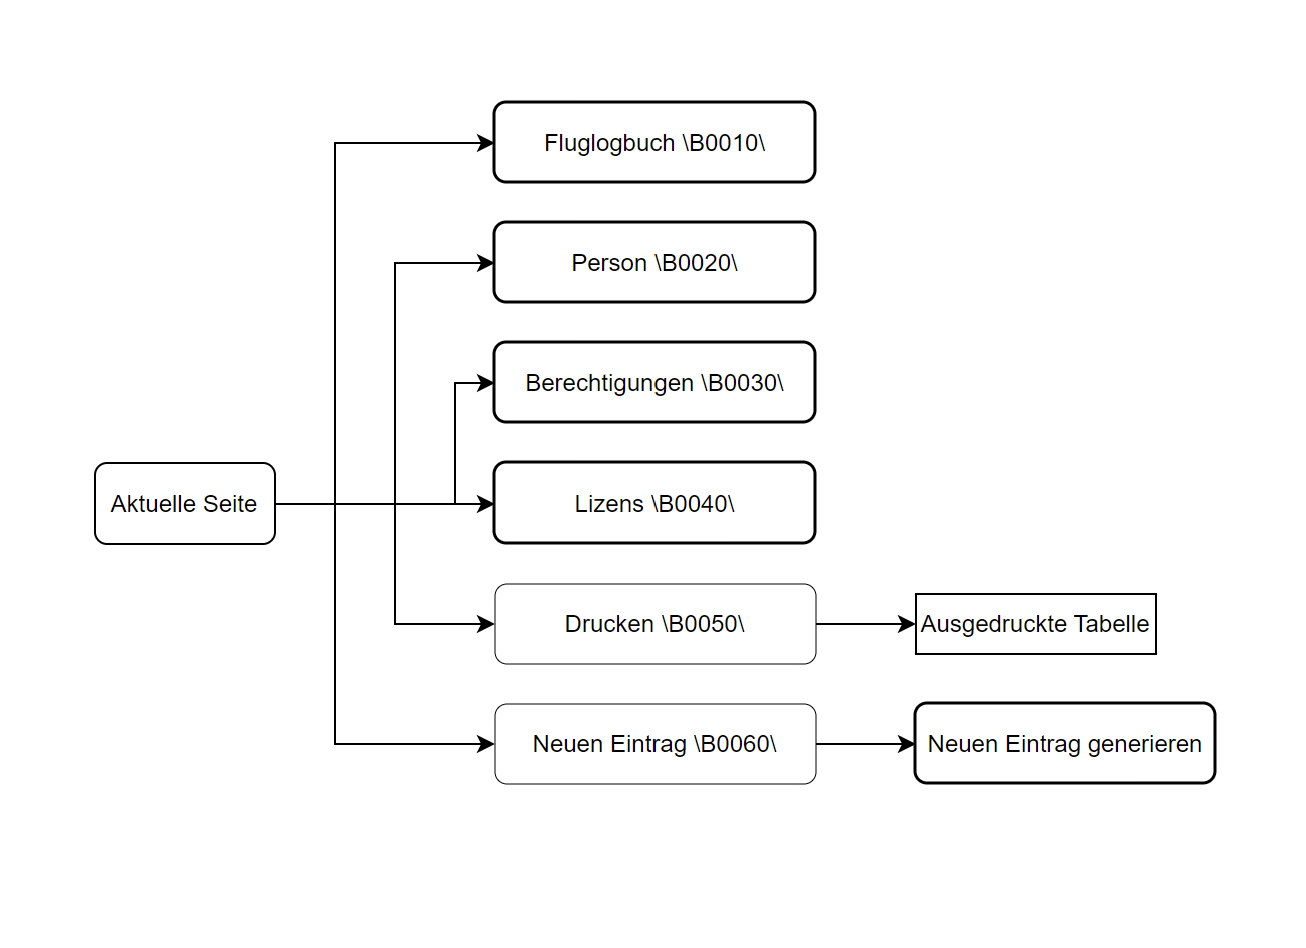
\includegraphics{Benutzeroberflaeche_Floglogbuch.png}
        \caption{Die Abbildung repräsentiert alle 4 Seiten}
        \label{fig:my_label}
    \end{figure}
    \pagebreak
    \subsubsection{Neuen Eintrag}
    \vspace{0.5cm}
    Im folgenden ist der Aufbau der Seite \glqq{}Neuen Eintrag\grqq{} modelliert.
    \begin{figure}[h!]
        \centering
        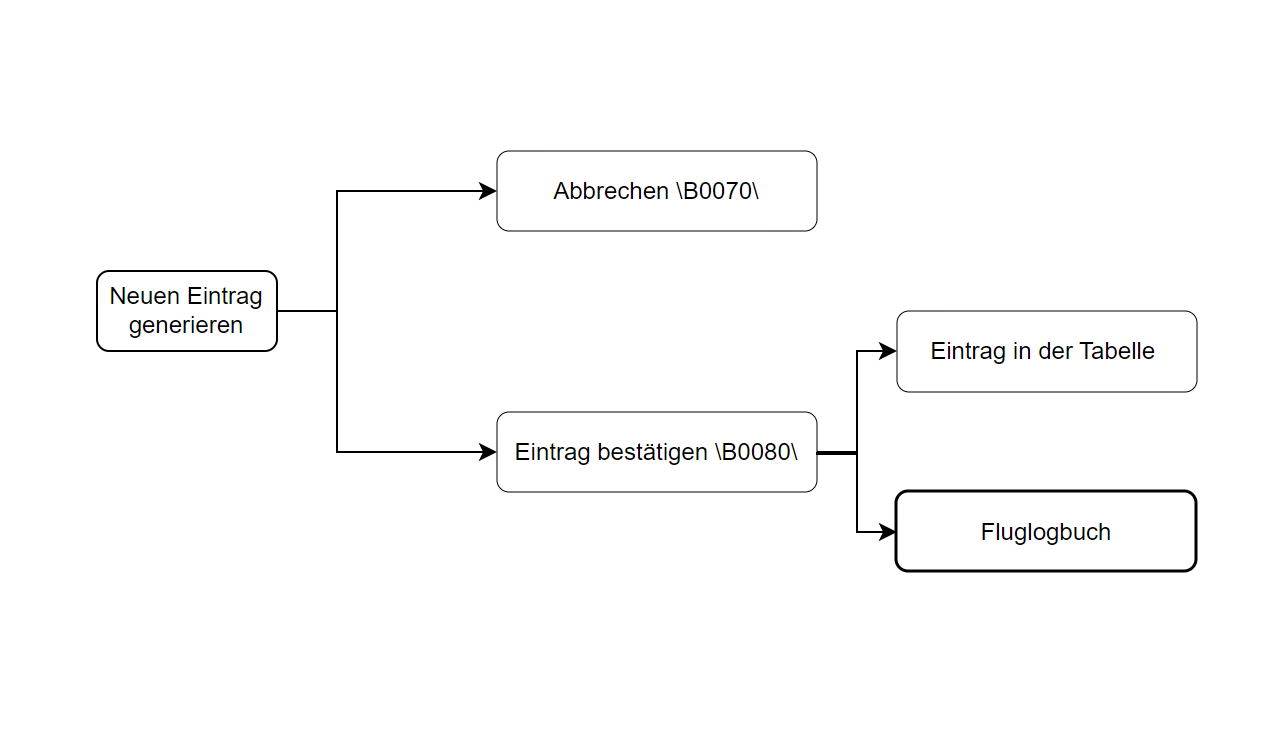
\includegraphics{Benutzeroberflaeche_Neuer_Eintrag.png}
        \caption{Neuen Eintrag}
        \label{fig:my_label}
    \end{figure}
    \vspace{0.5cm}

    \subsection{Glossar}
    \vspace{1cm}
    \begin{itemize}
    \item PIC - Person in control
    \begin{itemize}
        \item Das beschreibt die Person die das Flugzeug fliegt.
    \end{itemize}
    \item SEP - Single Engine Pistion
    \begin{itemize}
        \item Hiermit werden Flugzeuge beschrieben die ein maximales Abflugsgewicht von 5700 haben.
    \end{itemize}
    \item UL  - Ultraleicht 
    \begin{itemize}
        \item UL bezeichnet Flugzeuge, die mit maximal 450kg fliegen.
    \end{itemize}
    \item UTC - Universal Time Coordinated
    \begin{itemize}
        \item Das ist die koordinierte Weltzeit.
    \end{itemize}
    \end{itemize}
    
    \pagebreak

    \section{OOA-Modell}
    \begin{figure}[h!]
        \centering
        \rotatebox{270}{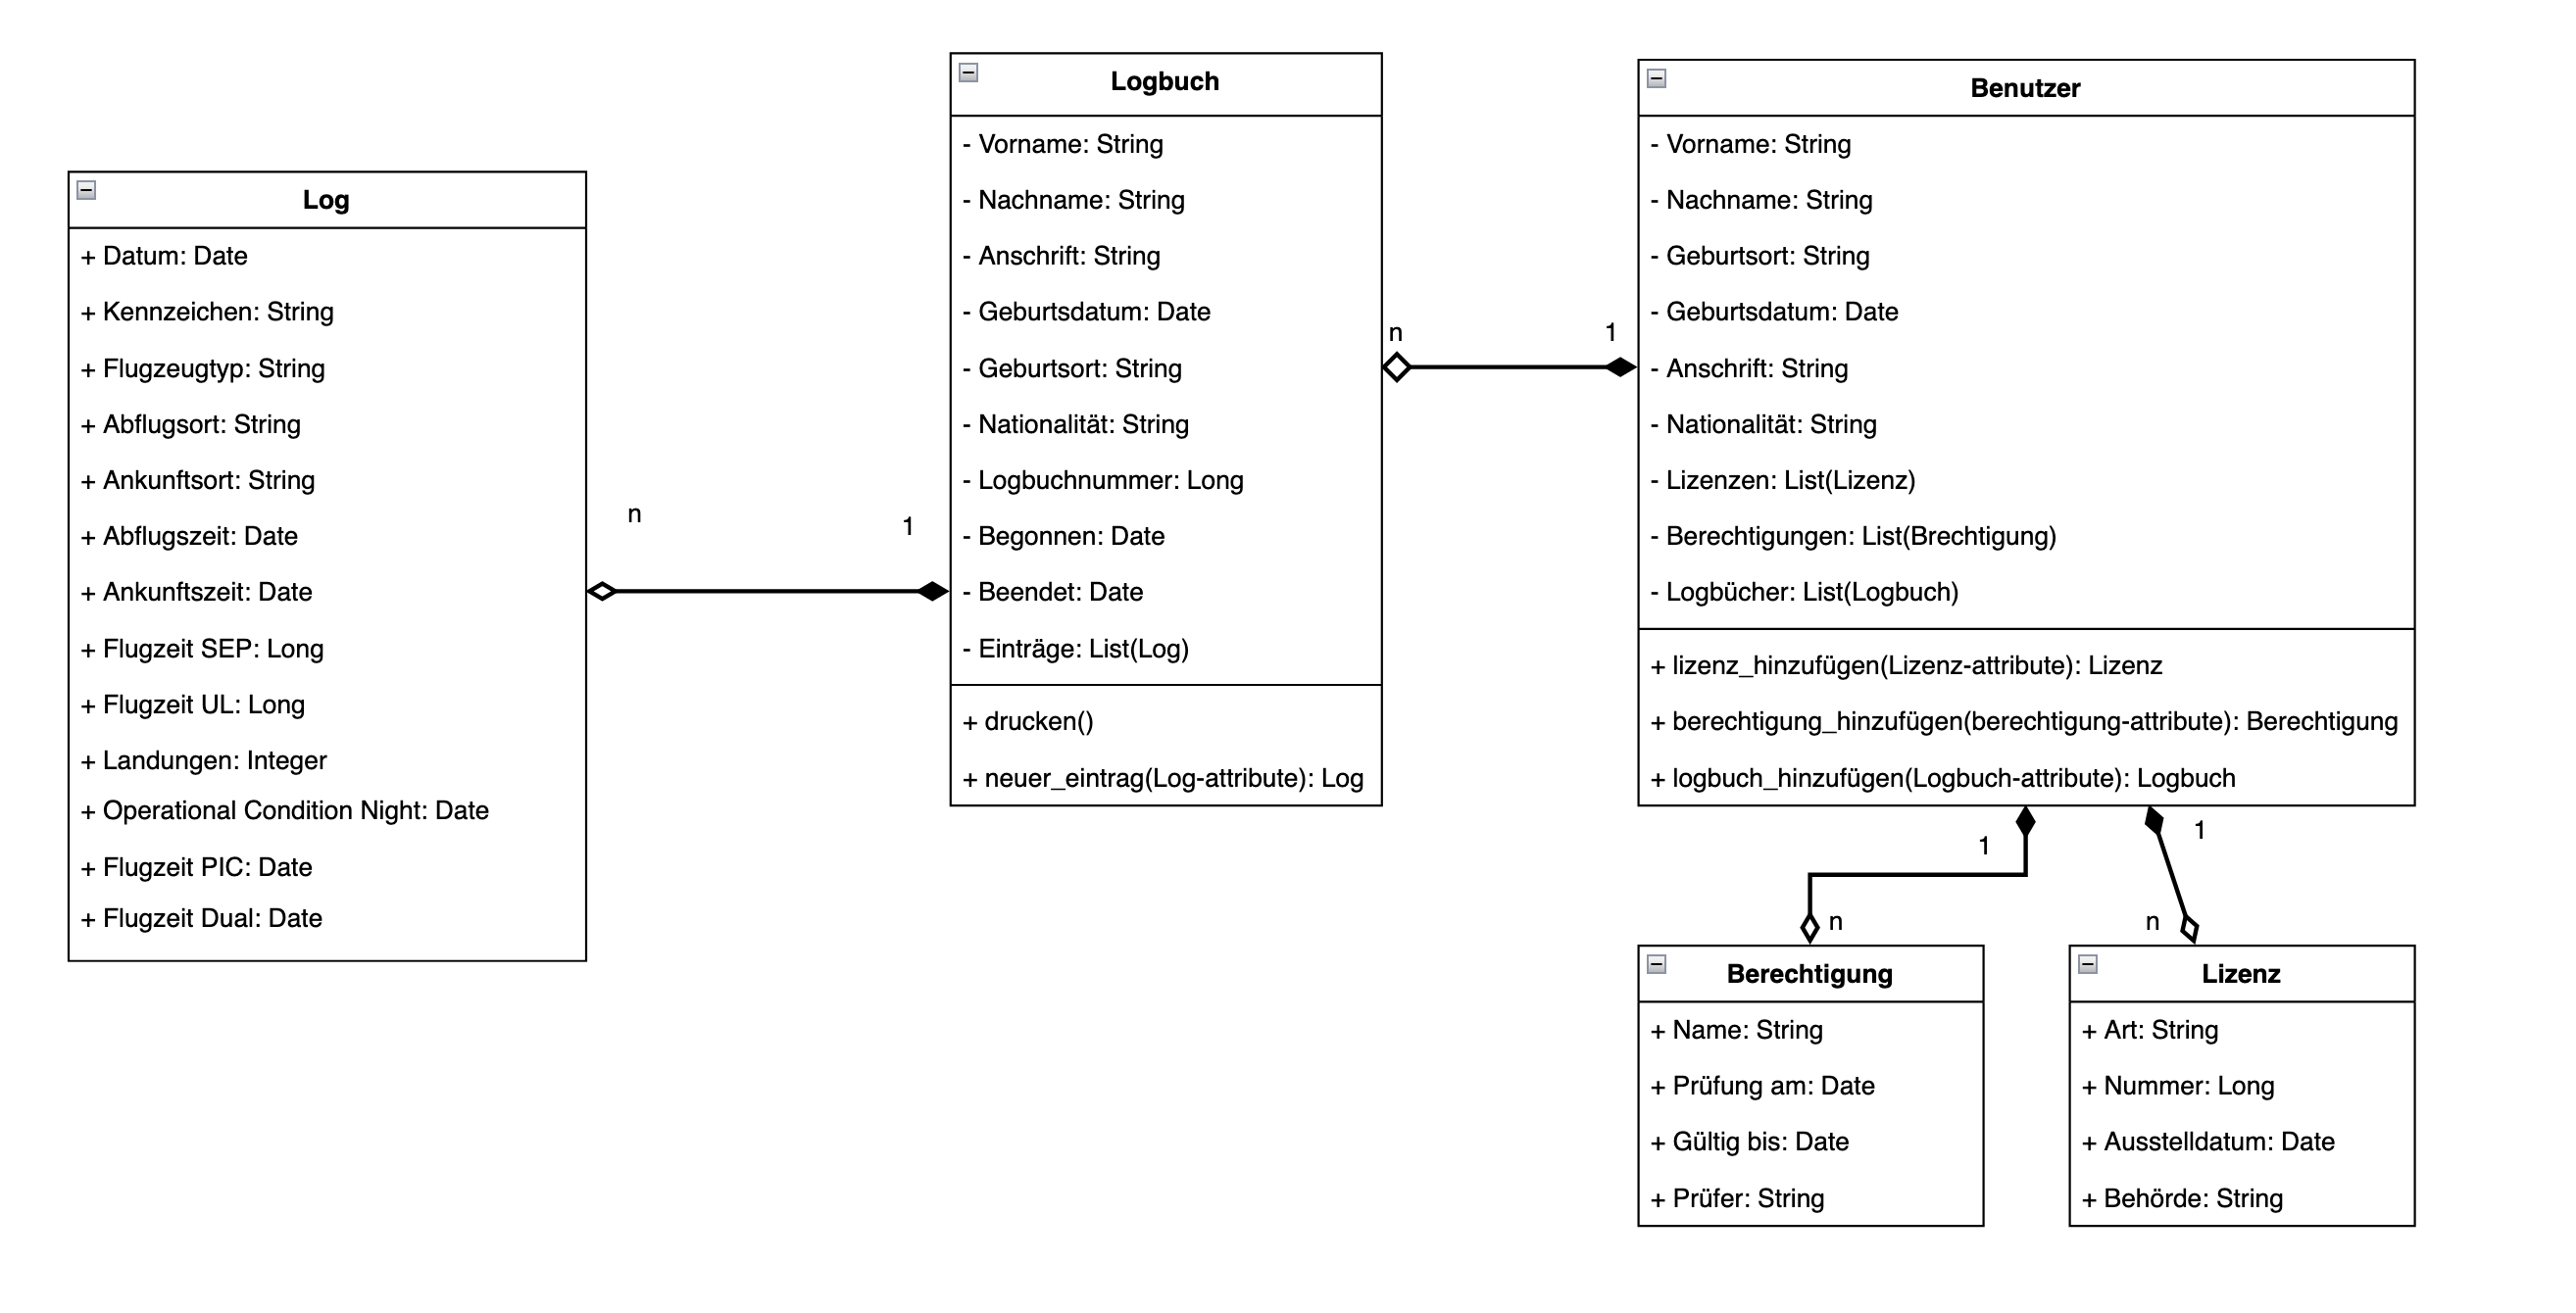
\includegraphics[width=21cm]{Abbildung_OOA.png}}
        \caption{OOA Modell}
        \label{fig:my_label}
    \end{figure}
    \pagebreak
    \noindent\\
    \noindent \textbf{Gedankengang:}\\
    
    \noindent Das Programm ist im ganzen Aufgeteilt in den Benutzer, die Lizenzen, die Berechtigungen, das Logbuch und die einzelnen Logs pro Flug. Die Lizenzen und Berechtigungen werden unter dem Benutzer gespeichert verwaltet und gelöscht. Das Fluglogbuch wird separat gehändelt und aus einzelnen Logs aufgebaut, die pro Flug dem Logbuch hinzugefügt werden.\\ Die Verwaltung der einzelnen Logbücher wird vom Benutzer aus gemacht, womit der Benutzer zur zentralen Verwaltungsklasse wird.

    \section{Konzept der Benutzerschnittstelle}
    \vspace{1cm}
    Um den Kunden einen sehr einfachen und sorglosen Start zu ermöglichen, haben wir als Entwickler uns gedacht, dass wir für den Kunden eine Anleitung schreiben, damit der Kunde schnellstmöglich auf die digitale Ebene wechseln kann. Als erstes müssen sie den Store Ihres Gerätes suchen, auf dem Sie die App nutzen wollen.\\ Je nachdem welches Endgerät Sie besitzen, müssen Sie den jeweiligen Store aufsuchen.\\ Nachdem Sie dies getan haben, geben Sie bitte den Namen der App in die Suchleiste Ihres Stores ein und suchen nach diesem. Kurze Zeit später sollte die App, die Sie gesucht haben, erscheinen und genau dieses installieren Sie auf dem Gerät Ihrer Wahl. \\Nach der ganzen Installation der App können Sie diese per Knopfdruck öffnen und dann bereits die von uns erstellten Felder sehen, die alle für Ihr Fluglogbuch wichtig sind. In der App können Sie Unter anderem per Knopfdruck auf den jeweiligen Button direkt zu Ihrer gewünschten Seite springen. Das bedeutet, wenn Sie zum Logbuch möchten, können Sie ganz einfach auf den Button mit der Beschreibung \glqq{}Logbuch\grqq{} drücken. Auf dieser Seite finden Sie den Button \glqq{}Neuen Eintrag\grqq{} wenn Sie den betätigen, gelangen Sie auf eine Neue Seit welche einfach aufgebaut ist, mit jeweils einem Textfeld pro Spalte in der Tabelle. Dann füllt ihr die Felder aus die ihr in die Tabelle schreiben wollt, drückt Bestätigen und schon wird automatisch für euch ein Tabelleneintrag generiert. \\
    \begin{figure}[h!]
        \centering
        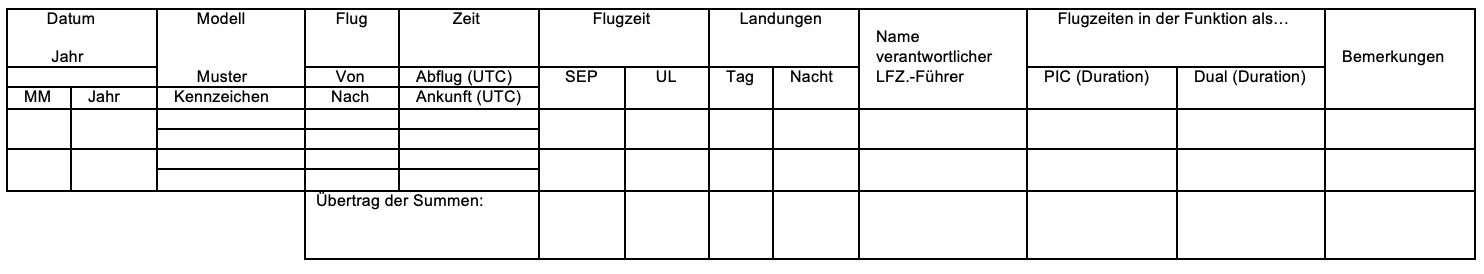
\includegraphics[width=17cm]{Logbuch.png}
        \caption{Fluglogbuch Tabelle}
        \label{fig:my_label}
    \end{figure}
    
    \noindent Um unsere App so einfach wie möglich für jeden zu gestalten, haben wir uns überlegt, dass wir zu jedem Punkt eine kurze Anleitung erstellen, damit Jung und Alt alle verlangten Daten verstehen. In der ersten Spalte sehen Sie, dass das Datum von Ihnen verlangt wird. Sie müssen wie in der Spalte aufgefordert das Jahr sowie den jeweiligen Tag und Monat, an dem Sie das Logbuch schreiben, angeben. \\
    In der zweiten Spalte wird von Ihnen verlangt, das Modell des Flugzeugs sowie das jeweilige Kennzeichen anzugeben. In der dritten und vierten Spalte wird von Ihnen verlangt, dass Sie einmal angeben, von wo Sie aus fliegen und wohin Sie fliegen möchten. In der vierten Spalte wird von Ihnen verlangt, dass Sie die Uhrzeit angeben, wann Sie losfliegen, aber nicht in Ihrer lokalen Zeitzone, sondern immer in der UTC-Zeitzone.\\ In der fünften Spalte müssen Sie eintragen, wie lange Sie mit einem bestimmten Flugzeugtypen geflogen sind. Unter anderem wird hier zwischen SEP und UL unterschieden. Mit SEP sind Flugzeuge gemeint, die ein maximales Abfluggewicht von etwa 5.700 Kilogramm haben. Mit UL meint man ein Flugzeug, welches ein Abfluggewicht von maximal 450 Kilogramm hat. \\
    
    \pagebreak
    
    \noindent In der sechsten Spalte wird von Ihnen verlangt, dass Sie Ihren Namen eintragen, nicht nur Ihren Vornamen, sondern auch den Nachnamen. In der vorletzten und siebten Spalte wird verlangt, dass Sie einmal die Zeit eintragen, welche Sie persönlich geflogen sind. Dies wird unter PIC gekennzeichnet. Unter Dual versteht man in diesem Fall, dass der Pilot noch eine Begleitperson dabei hatte. Von dieser Person muss man auch die jeweilige Flugzeit eintragen, falls die Person auch geflogen ist. In der letzten Spalte wird von Ihnen verlangt, dass Sie eine Bemerkung schreiben, falls es zum Beispiel während des Fluges zu starkem Nebel gekommen ist.\\
    
    \begin{figure}[h!]
        \centering
        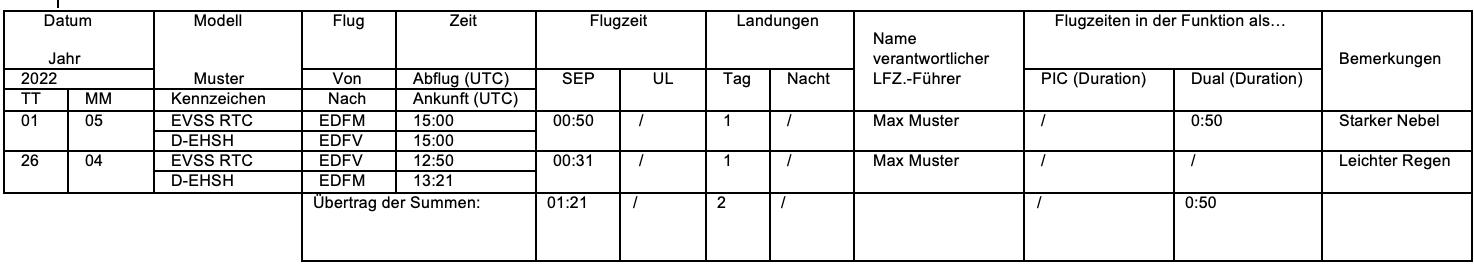
\includegraphics[width=17cm]{Logbuch_Beispiel.png}
        \caption{Fluglogbuch Beispielstabelle}
        \label{fig:my_label}
    \end{figure}
    \begin{figure}[h!]
        \centering
        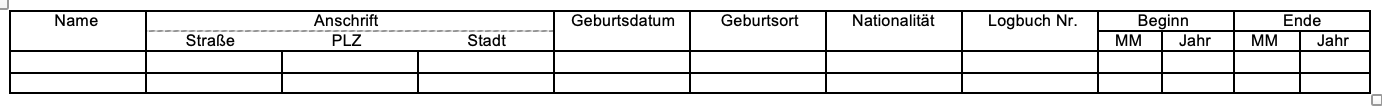
\includegraphics[width=17cm]{Personen.png}
        \caption{Personen Tabelle}
        \label{fig:my_label}
    \end{figure}
    
    \noindent In der Tabelle, in der Sie Angaben zu Ihrer Person machen, müssten Sie Ihren Namen, Ihre Straße, Postleitzahl, Stadt, Geburtsdatum, Geburtsort, Ihre Nationalität, Ihre Logbuch-Nummer sowie den Zeitraum eintragen, in dem Sie das Logbuch begonnen und beendet haben.
    \begin{figure}[h!]
        \centering
        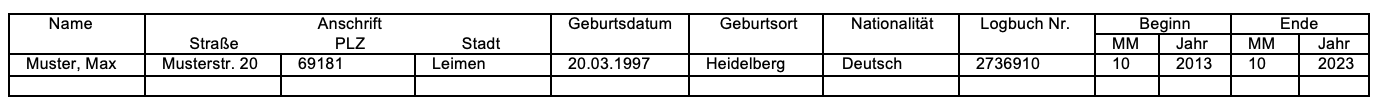
\includegraphics[width=17cm]{Personen_Beispiel.png}
        \caption{Personen Beispielstabelle}
        \label{fig:my_label}
    \end{figure}

    \begin{figure}[h!]
        \centering
        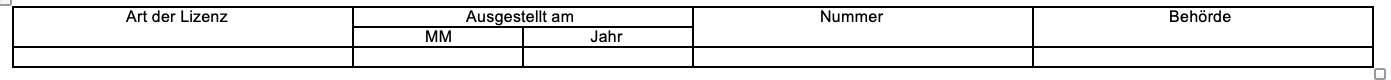
\includegraphics[width=17cm]{Lizenz.png}
        \caption{Lizenz Tabelle}
        \label{fig:my_label}
    \end{figure}
    
    \noindent In dieser Tabelle geht es um Ihre erworbene Lizenz, und zwar müssten Sie einmal eintragen, welche Lizenz Sie erworben haben, beziehungsweise welche weiteren Lizenzen. Nachdem Sie dies getan haben, geht es weiter mit dem Ausstellungsdatum Ihrer Lizenz, heißt einmal den Monat und einmal das Jahr. Nach all diesen Schritten müssten Sie in den nächsten zwei Spalten einmal die Nummer Ihrer Lizenz eintragen und bei welcher Behörde Sie diese erworben haben.\\
    
    \begin{figure}[h!]
        \centering
        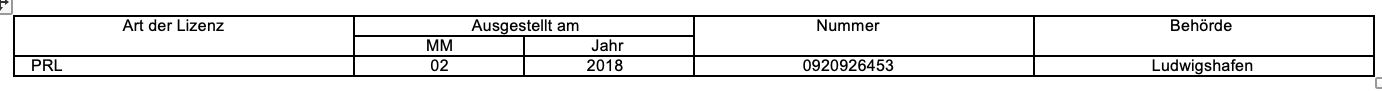
\includegraphics[width=17cm]{Lizenz_beispiel.png}
        \caption{Lizenz Beispielstabelle}
        \label{fig:my_label}
    \end{figure}

    \begin{figure}[h!]
        \centering
        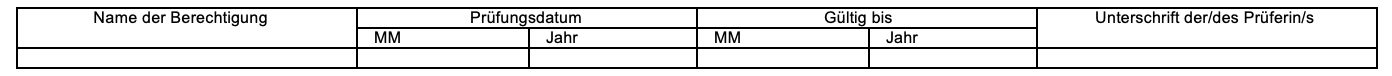
\includegraphics[width=17cm]{Berechtigung.png}
        \caption{Berechtigung Tabelle}
        \label{fig:my_label}
    \end{figure}

    \pagebreak
    
    \noindent In dieser Tabelle müssen Sie einmal den Namen Ihrer Berechtigung eintragen, sowie wann Sie die Prüfung abgelegt haben und bis wann Ihre Berechtigung gültig ist. Die Angaben erfolgen, indem Sie den jeweiligen Monat sowie das jeweilige Jahr angeben. Aber das ist nicht die einzige Sache, die Sie in die Tabelle eintragen müssen, Sie müssen noch dafür sorgen, dass Ihr Prüfer oder Ihre Prüferin ebenfalls unterschreibt.\\
    
    \begin{figure}[h!]
        \centering
        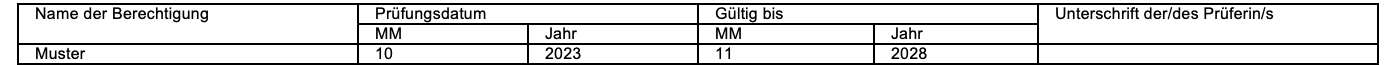
\includegraphics[width=17cm]{Berechtigung_Beispiel.png}
        \caption{Berechtigung Beispielstabelle}
        \label{fig:my_label}
    \end{figure}
    
    \section{OOD-Modell}

    \vspace{1cm}
    \noindent \textbf{Gedankengang:}\\
    \noindent \vspace{0.5cm} \\
    \noindent Das Modell zeigt den Aufbau der App und dessen Abläufe und Methoden. Enthalten sind alle Methoden die für den Aublauf und den Benutzer notwendig sind. \\Das Userinterface greift auf die Konfiguration und das Fluglogbuch zu. Über die Konfiguration können die Daten des Benutzers und dessen Logs gespeichert geändert und geladen werden.\\ Die Aufteilung der Klassen Benutzer, Lizenz und Berechtigung unter Konfiguration setzt zum Ziel, dass die Informationen für die Entwickler und für die Kunden unter den Optionen erreichbar sind. Der Hauptpart mit dem Fluglogbuch ist separat und wird unter dem Benutzer gespeichert.
    \pagebreak
    
    \begin{figure}[h!]
    \centering
    \rotatebox{270}{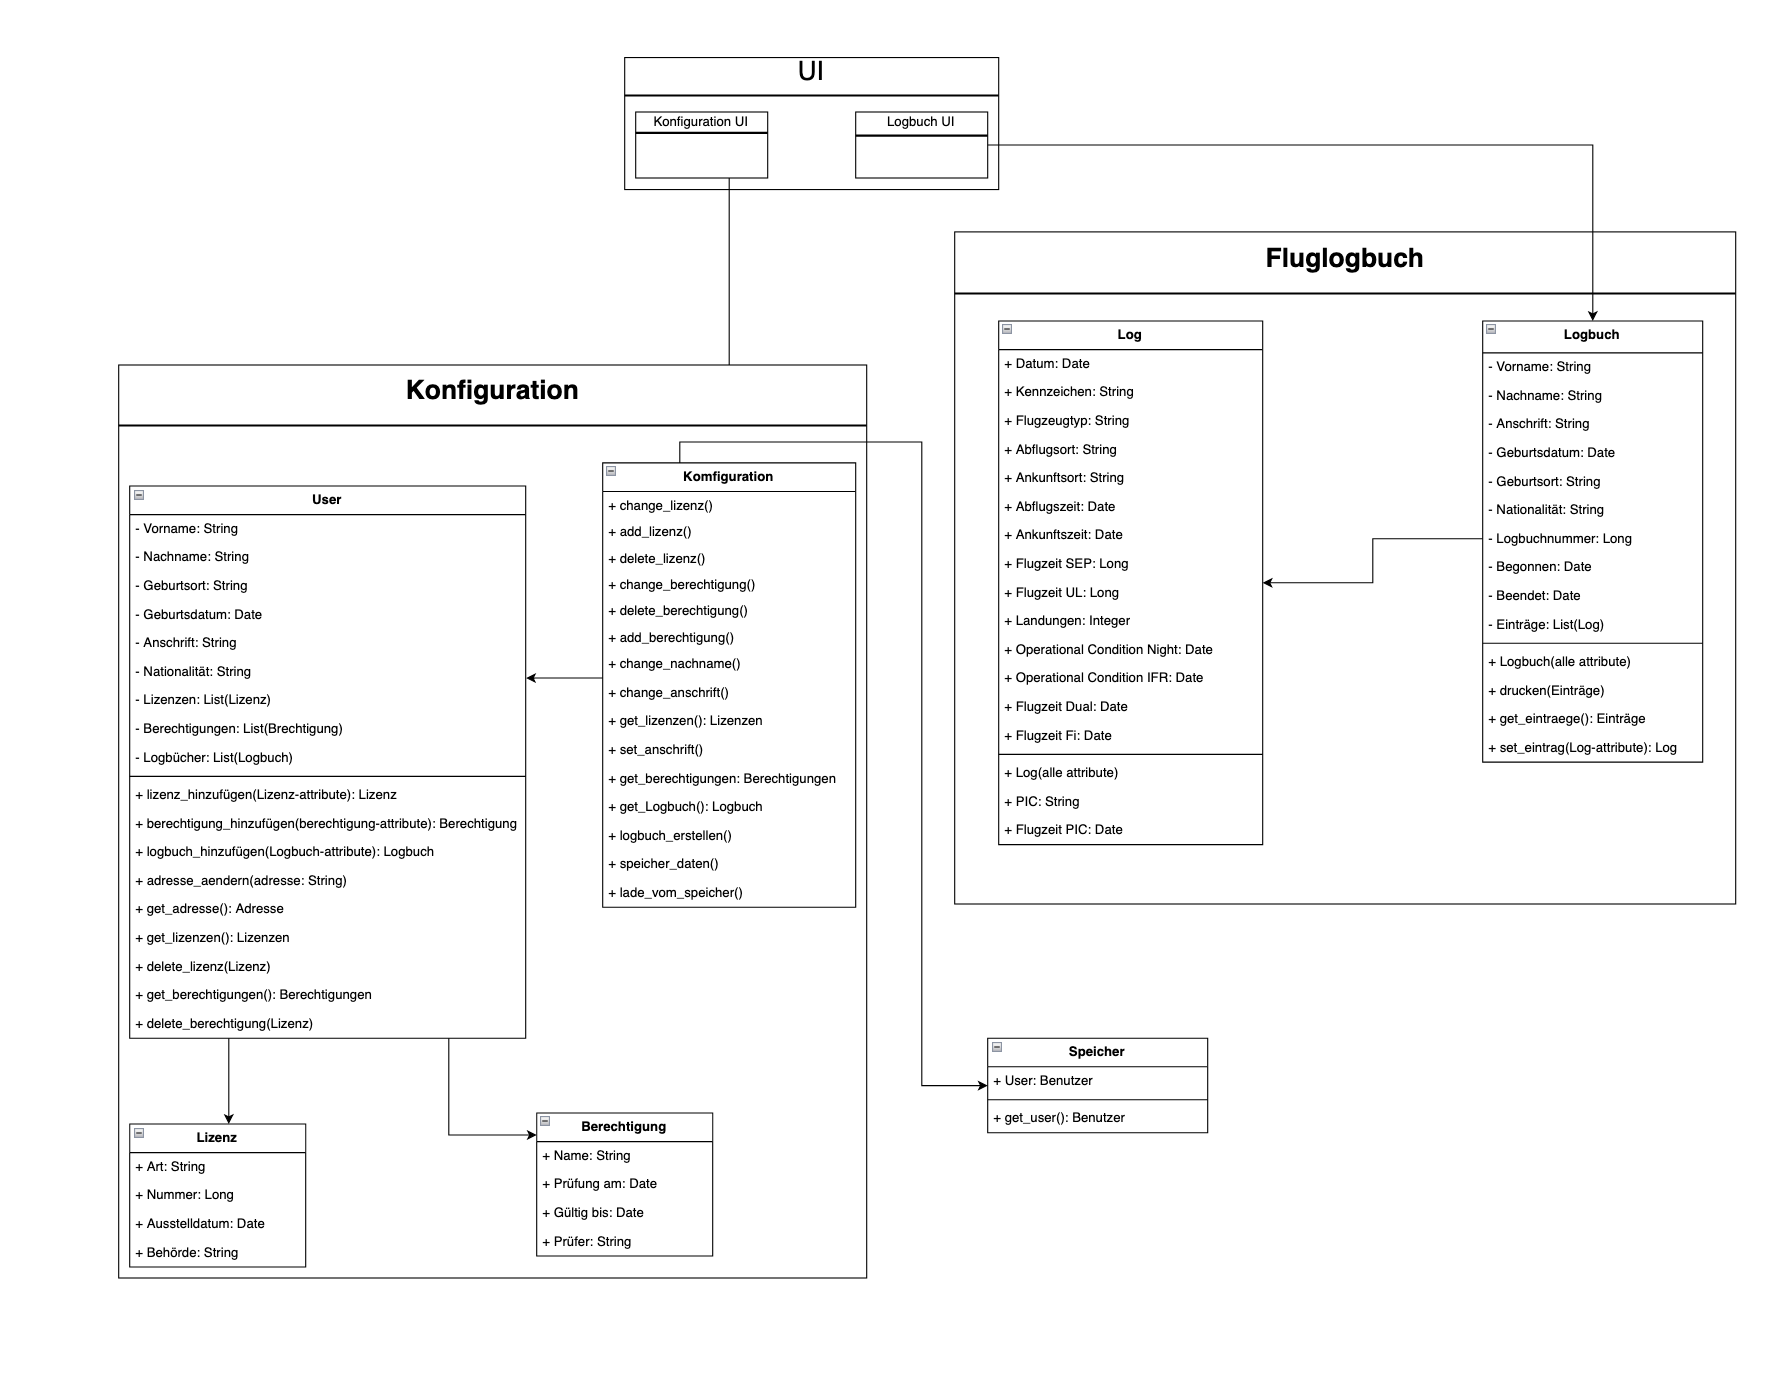
\includegraphics[width=21cm]{OOD_Abbildung.png}}
    \caption{OOD Model}
    \label{fig:my_label}
    \end{figure}
    \pagebreak

\end{document}